\documentclass[11pt, oneside]{article} 
\usepackage{geometry}
\geometry{letterpaper} 
\usepackage{graphicx}
	
\usepackage{amssymb}
\usepackage{amsmath}
\usepackage{parskip}
\usepackage{color}
\usepackage{hyperref}

\graphicspath{{/Users/telliott_admin/Tex/png/}}
% \begin{center} 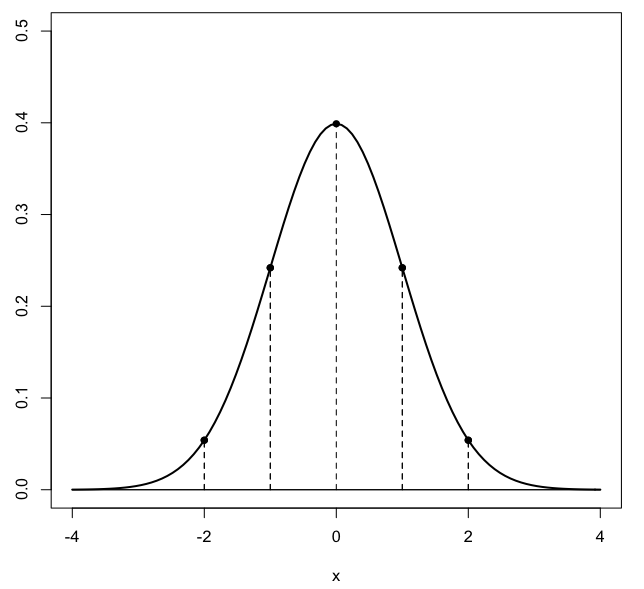
\includegraphics [scale=0.4] {gauss3.png} \end{center}

\title{Nahin Imaginary Tale Ch. 1}
\date{}

\begin{document}
\maketitle
\Large
Nahin gives this problem from Diophantus:  a right triangle has area $7$ and perimeter $12$.  Find the lengths of the two sides.  

From these constraints, write:
\[ ab = 14 \]
\[ a + b + \sqrt{a^2 + b^2} = 12 \]

\subsection*{analysis}
Suppose the triangle is isosceles. Then $a = b$ and
\[ a^2 = 14 \]
\[ a = \sqrt{14} \approx 3.74 \]

Then we must have
\[ c^2 = a^2 + b^2 =  14 + 14 = 28 \]
\[ c = 5.29 \]
The perimeter would be approximately
\[ 3.74 + 3.74 + 5.29 = 12.77 \]
This perimeter is too long.  But an isosceles triangle has the \emph{shortest} perimeter for a given area.  Hence, there is no solution.

\subsection*{my solution}
\[ a + b + \sqrt{a^2 + b^2} = 12 \]
Solve this algebraically.  First, remove the square root.
\[ a^2 + b^2 = (12 - a - b)^2 \]
\[ = 12^2 - 12a -12b -12a + a^2 + ab - 12b + ab + b^2 \]
Cancel $a^2$ and $b^2$
\[ 0 = 12^2 - 12a -12b -12a + ab - 12b + ab \]
\[ = -24a - 24b + 2ab + 12^2 \]
\[ = -12a - 12b + ab + 72 \]
Substitute for $b$ from $ab = 14$:
\[ = -12a - 12 \frac{14}{a} + 14 + 72 \]
\[ -12a^2 + 86a - 168 = 0 \]
Factor out $-2$
\[ 6a^2 - 43a + 84 = 0 \]
\[ a = \frac{43 \pm \sqrt{43^2 - 4 \cdot 6 \cdot 84}}{12} \]
\[ = \frac{43 \pm \sqrt{1849 - 2016}}{12} \]
\[ = \frac{43 \pm \sqrt{-167}}{12}  \]
There is no real solution.

\subsection*{Diophantus solution}
Nahin says a bright idea is to substitute:
\[ a = \frac{1}{x} \]
\[ b = 14x \]
so then
\[ a + b + \sqrt{a^2 + b^2} = 12 \]
\[ \frac{1}{x} + 14x + \sqrt{\frac{1}{x^2} + 14^2 x^2} = 12 \]
Nahin says this is \textbf{easily} put in the form
\[ 172x = 336 x^2 + 24 \]

Easily?  We have the same problem with the square root as before.  Multiply by $x$
\[ 1 + 14x^2 + \sqrt{1 + 14^2 x^4} = 12x \]
Now isolate the square root and square the terms on the other side
\[ (-14x^2 + 12x - 1)^2 \]
\[ = 14^2 x^4 -(14)12x^3 + 14x^2 -(14)12x^3 + 144x^2 - 12x + 14x^2 - 12 x + 1 \]
The two terms from squaring $\sqrt{1 + 14^2 x^4}$ disappear, leaving:
\[ 0 =  -(14)12x^3 + 14x^2 -(14)12x^3 + 144x^2 - 12x + 14x^2 - 12 x  \]
\[ =  -2(14)12x^3 + 28x^2  + 144x^2 - 24x    \]
\[ -336 x^3 + 172x^2 - 24x = 0 \]
Divide by $x$
\[ -336 x^2 + 172x - 24 = 0 \]
Make all terms positive
\[ 336 x^2 + 24 = 172x \]
This matches what Nahin has.

Remove a factor of $4$
\[ -84 x^2 + 43x - 6 = 0 \]

We have still to solve for $x$ and then go back to $a$ and $b$.  But we cannot solve for $x$, because the discriminant is
\[ 43^2 - 4 \cdot 84 \cdot 6 = 1849 - 2016 = - 167  \]
that is, less than zero.  So again, there are no real solutions.

\subsection*{compare solutions}

Suppose we do write
\[ x = \frac{-43 \pm \sqrt{-167}}{2 (-84)} \]
and compare with
\[ a =  \frac{43 \pm \sqrt{-167}}{12}  \]
How does this make sense in light of the substitution $a = 1/x$?  How can we have the same value in the numerator of both expressions, when they are inverses?

Recall that for complex numbers
\[ \frac{1}{z} = \frac{z*}{zz*} \]

Taking the positive root of $x$
\[ x =  \frac{-43 + \sqrt{-167}}{2 (-84)} \]
\[ = \frac{43}{168} - \frac{\sqrt{-167}}{168} \]
\[ x* =  \frac{43}{168} + \frac{\sqrt{-167}}{168} \]
and 
\[ xx* = \frac{43^2}{168^2} + \frac{167}{168^2} \]
Hence
\[ \frac{1}{x} = \frac{x*}{xx*} = \frac{43/168 + \sqrt{-167}/168}{43^2/168^2 + 167/168^2} \]
\[ = \frac{43 + \sqrt{-167}}{43^2/168 + 167/168} \]

The numerators match now.  The denominator in the last expression is
\[ \frac{43^2}{168} + \frac{167}{168} \]
\[ 43^2 + 167 = 1849 + 167 = 2016 \]
But
\[ 12 \times 168 = 2016 \]
So the denominators match, as well.

\end{document}